
%%%%Présentation#####


\section{Introduction}
\subsection{Contexte}




\begin{frame}{La sécurité alimentaire } 
\setbeamercovered{invisible}
%  \frametitle{La sécurité alimentaire \rlap{\raisebox{-\dp\strutbox}{\includegraphics[height=\baselineskip]{monde}}}}

\begin{columns}

 \begin{column}{.65\textwidth}
  \begin{outline}
\begin{itemize}[itemsep=10pt]
\item {Plan de développement durable de l'ONU et ses  objectifs principaux : \hspace{15mm} 
\includegraphics[width=0.6\linewidth]{ONU-removebg-preview}}
\vspace{-4mm}
               \begin{flushleft}
             \textcolor{myblue1}{{\tiny\href{https://www.un.org/sustainabledevelopment/fr/objectifs-de-developpement-durable/}{https://www.un.org/sustainabledevelopment/fr/objectifs-de-developpement-durable/}}}  
\end{flushleft}  

        \begin{itemize}[itemsep=8pt,label=$\rightarrow$]
      \item{ Éliminer la faim dans le monde ({\small Faim zéro}) }   
 \item Nourrir une population croissante
              \item Préserver l'environnement%  \\[-8mm](développer une agriculture  durable)  \hspace{15mm} 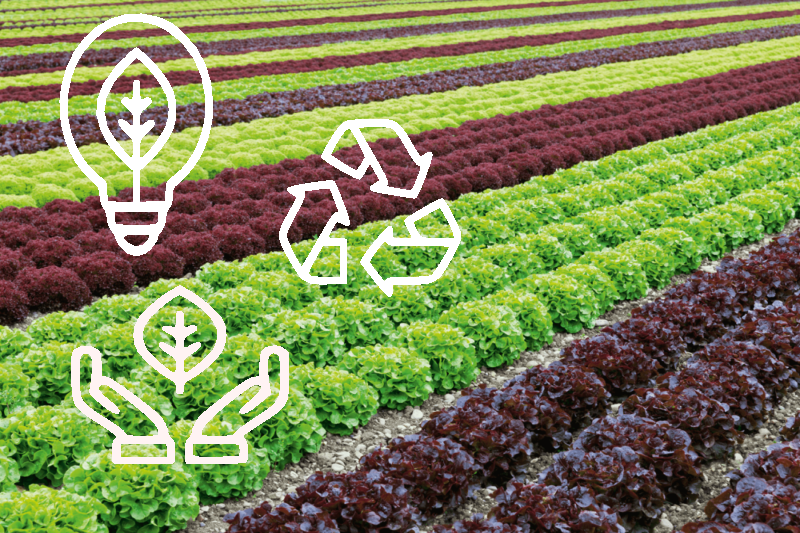
\includegraphics[width=0.16\linewidth]{mono}}
\end{itemize}
\end{itemize}
\end{outline} 
 \end{column}

 \begin{column}{.4\textwidth} 
 \vspace{14mm}
            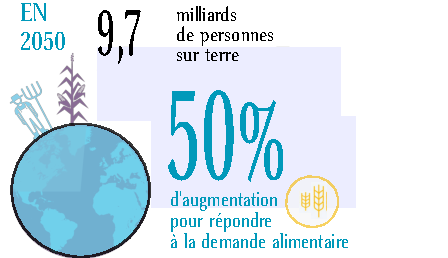
\includegraphics[width=1\linewidth]{doubler_rendement}         
 \end{column}
       

\end{columns} 



\pause
\begin{columns}

 \begin{column}{.65\textwidth}
 \begin{outline}
	\begin{itemize}[itemsep=5pt]
	\item Pour assurer la demande alimentaire plusieurs solutions :
	
        \begin{itemize}[itemsep=6pt, label=$\rightarrow$] 
    \item Limiter le gaspillage alimentaire         
	  \item Limiter les pertes de rendements 
	\end{itemize} 
\end{itemize}
\end{outline}
 \end{column}
  \pause
 \begin{column}{.4\textwidth} 
\hspace{5mm}

\vspace{-7mm}
 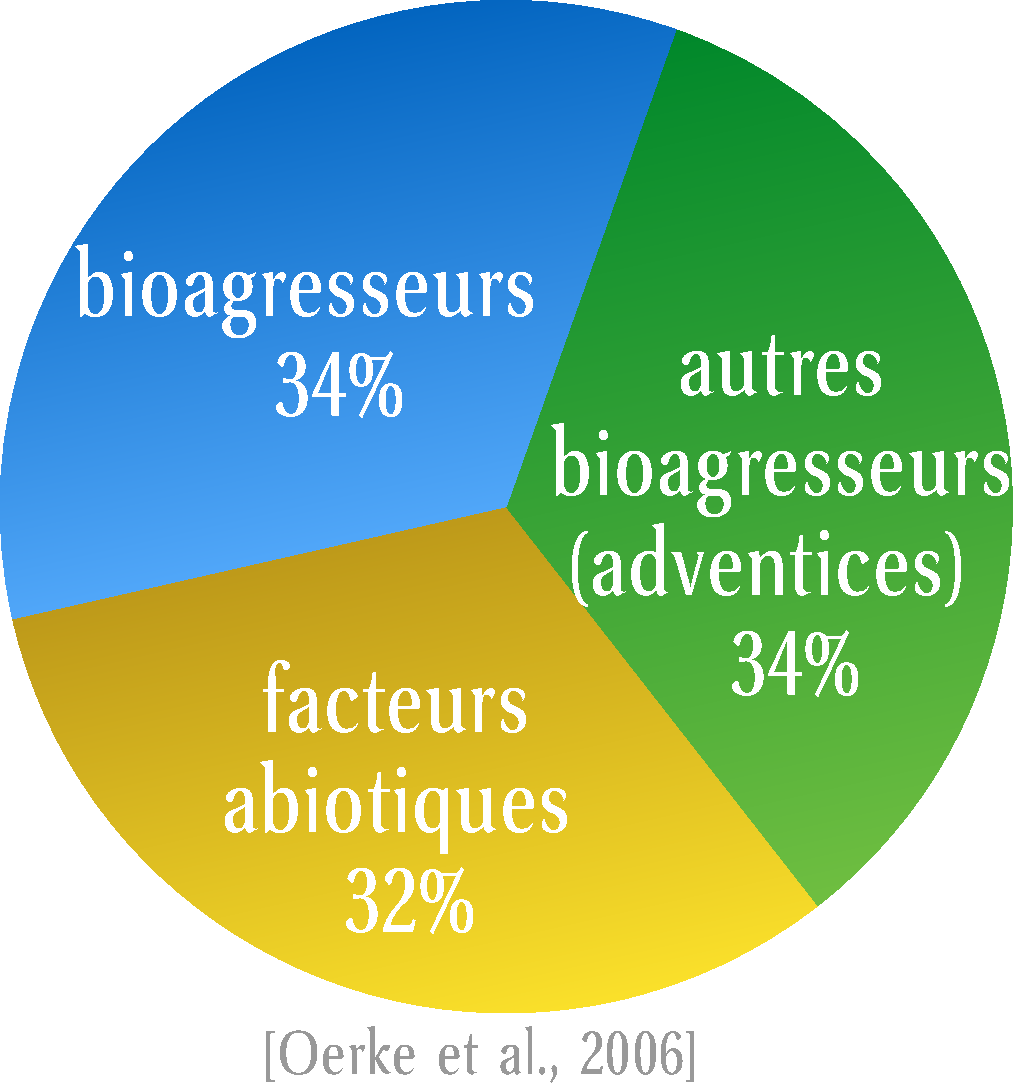
\includegraphics[width=.60\linewidth]{croplosses0} 
 \end{column}
\end{columns}
           
\end{frame}                                                                                                                                                    

\begin{frame}{Impacts des  bioagresseurs}


\begin{outline}
\begin{itemize}[itemsep=10pt]
\item  Jusqu'à 68 \% de pertes de rendement à l'échelle mondiale \textcolor{shadecolor}{{\small[Oerke \textit{et al.,} 2006]}}\\

               
      \hspace{15mm}
            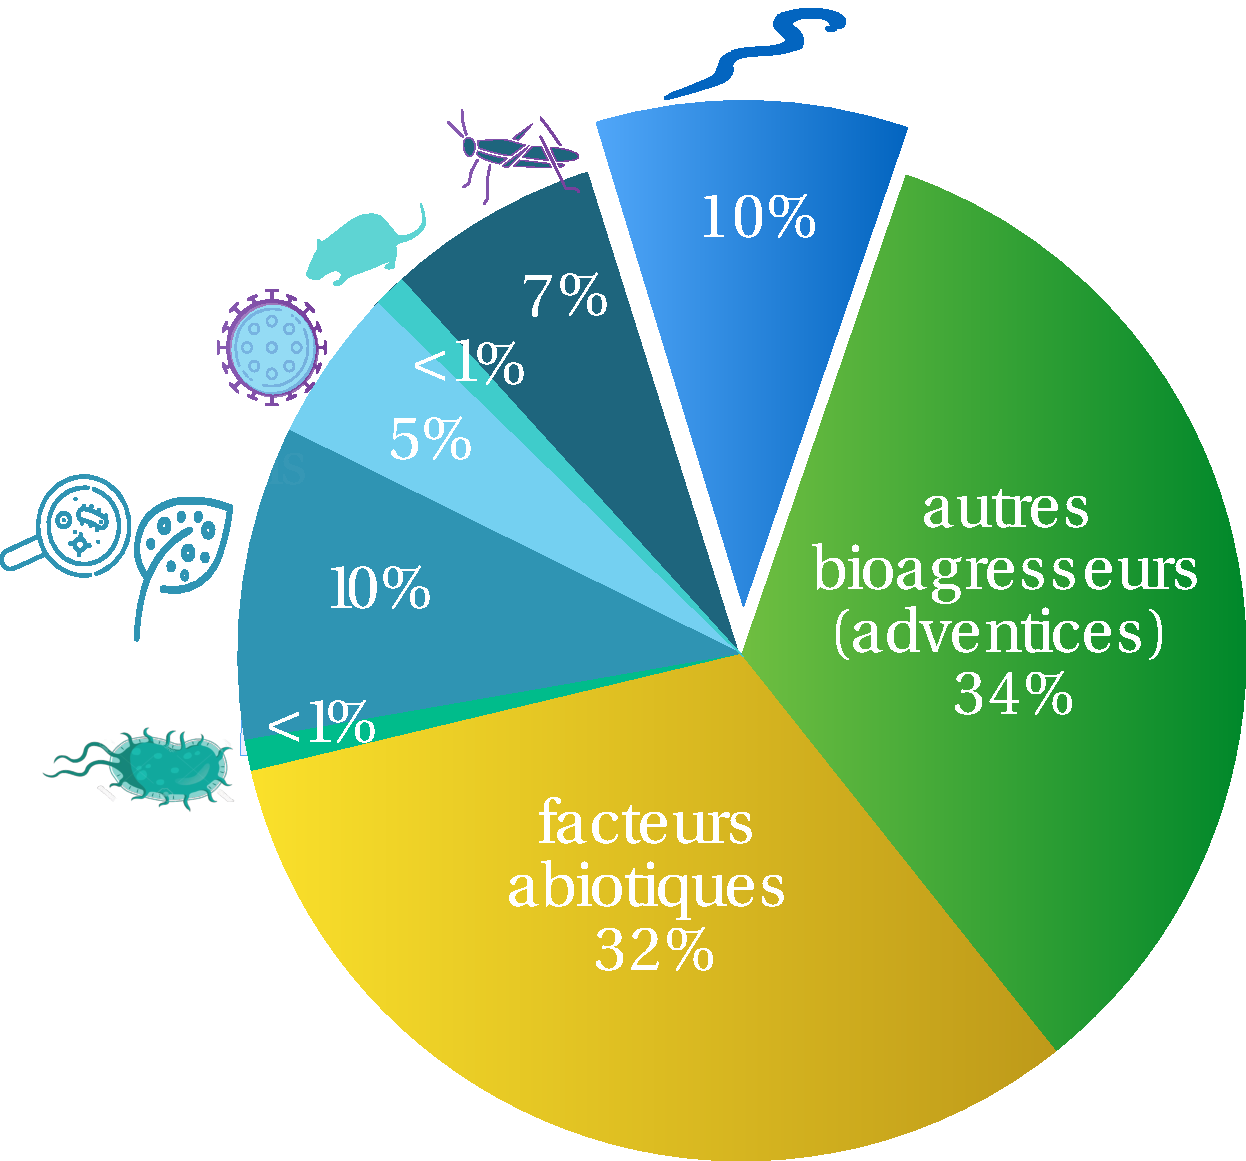
\includegraphics[width=0.6\linewidth]{croplosses2}
        
               \vspace{-5mm}
 \item \textcolor{myblue2}{Nématodes phytoparasites} : 10 \% de pertes de rendements à l'échelle mondiale,    > 100 milliards d'\euro{}/an \textcolor{shadecolor}{{\small[Chitwood \textit{et al.,} 2003]}} 
\end{itemize}
\end{outline}
\end{frame}                                                                                                                                                    



%
%\begin{frame}{Introduction}
%
%
%\begin{itemize}[itemsep=15pt]
%\item En 2050, la population > 9 milliards $\Rightarrow$ le rendement agricole devra doubler par rapport à aujourd'hui pour répondre à la demande alimentaire.
%\item Cependant le rendement agricole stagne voir diminue (30 à 40 \% de pertes annuelles) à cause de
%	\small{
%	\begin{itemize}
%	\item la diminution des sols cultivables, 
%	\item l’émergence de ravageur, maladies (Stukenbrock \textit{et al}., 2008),
%	\item limitation des pesticides.
%	\end{itemize}}
%	\pause
%\item Pour répondre à la demande des solutions alternatives et respectueuses de l'environnement existent :
%	\small{
%	\begin{itemize}
%	\item la lutte biologique, 
%	\item la diversification des cultures,
%	\item la résistance naturelle des plantes. 
%	\end{itemize}}
%\end{itemize}
%
%\begin{beamercolorbox}[sep=1mm,rounded=true]{darkbox}
%		\small\ding{229} Cette dernière et très prometteuse car c'est la méthode la plus économique et efficace parmi les solutions  respectueuse de l'environnement. 
%	\end{beamercolorbox}
%\end{frame}                                                                                                                                                    






\begin{frame}{Les nématodes phytoparasites}
\setbeamercovered{invisible}
\vspace{-0.1cm}
\begin{columns}

 \hspace{3mm}
 \begin{column}{.3\textwidth}

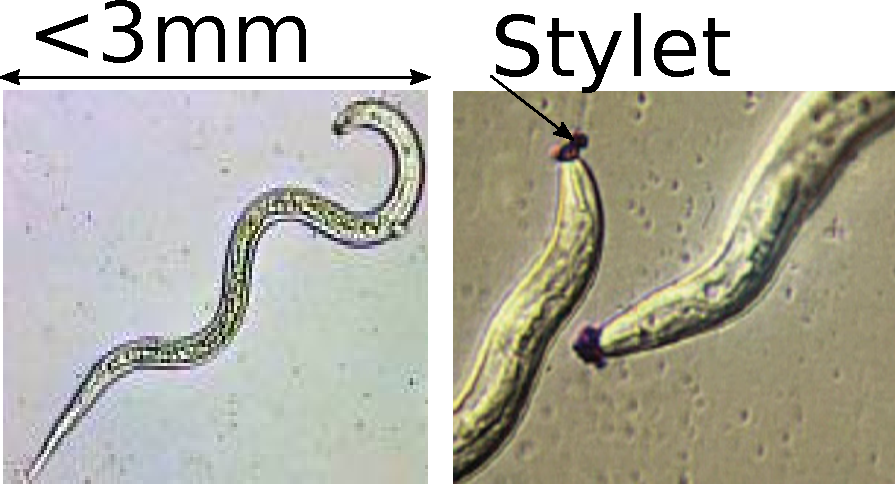
\includegraphics[width=0.7\linewidth]{nematode}    
 \end{column}

 \begin{column}{.8\textwidth} 

\begin{itemize}[leftmargin=-0.5cm]
\item Vers microscopiques
\item Plus de 4 000 espèces parmi 25 000 décrites \\ \textcolor{shadecolor}{{\small [Decraemer \& Hunt, 1986]}}
\end{itemize}

 \end{column}
\end{columns}

\vfill
\begin{columns}
\hspace{3mm}
 \begin{column}{.3\textwidth}     
 
\vspace{5mm}
  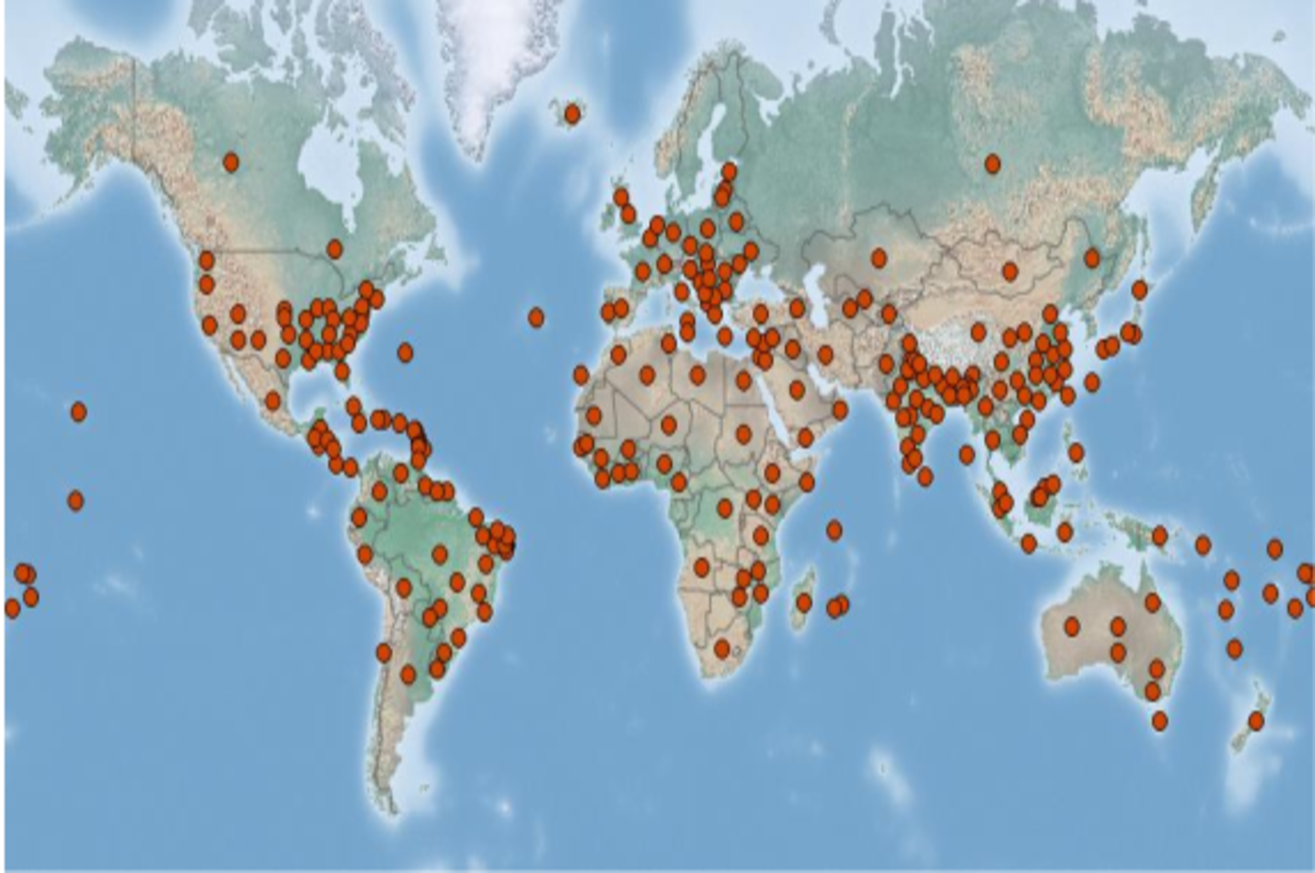
\includegraphics[width=.7\linewidth]{distributionM_incoginta} 
 \end{column}

 \begin{column}{.8\textwidth}
 \hspace{-5mm}\alert{ Ubiquistes et ravageurs :}
            \begin{itemize}[leftmargin=-0.5cm]
            
\item Les plus nuisibles $\Rightarrow$ les nématodes à galles \textit{(Meloidogyne spp.)} \\ 
 \textcolor{shadecolor}{{\small[ Jones \textit{et al.,} 2013]}}
\item Parasites racinaires obligatoires 

% \includegraphics[height=0.2\textheight]{incognita} 
            \end{itemize}
 \end{column}
\end{columns} 

\vspace{-0.5mm}

\begin{columns}
\hspace{1.7mm}
 \begin{column}{.3\textwidth}
 
  \begin{tikzpicture} 
\visible<1>{\node  (img1){ \phantom{\includegraphics<1>[width=0.7\linewidth]{melo}}};}
\visible<2>{\node (img1.south) {\includegraphics<2>[width=0.7\linewidth]{melo}};}
 \end{tikzpicture} 
          
 \end{column}
 \begin{column}{.8\textwidth}
 \hspace{-7mm}
            \begin{itemize}[leftmargin=-0.38cm]
           
\item<2>  Extrêmement polyphages : plus de 5500 espèces \\de plantes \textcolor{shadecolor}{{\small[Blok \textit{et al.,} 2008]}}  
\item<2> Plus de 40 \%  des exploitations en culture maraîchère \\ touchées en région PACA  \textcolor{shadecolor}{{\small[Djian-Caporalino \textit{et al.,} 2012]}}                  
\item<2> \textit{M. incognita}  l'espèce la plus répandue dans le monde et \\dans le Sud de la France \textcolor{shadecolor}{{\small[Djian-Caporalino \textit{et al.,} 2012]}}   
            \end{itemize}
 \end{column}
\end{columns}        
\end{frame}

\subsubsection{Cycle de vie}


\begin{frame}{Cycle de vie de \textit{M. incognita}}


\setbeamercovered{invisible}
\vspace{-0.1cm}
\begin{columns}
 \begin{column}{.5\textwidth}
            \begin{itemize}[leftmargin=0.75cm,itemsep=10pt]
\item  4 stades de développement de l’œuf à l'adulte
\onslide<2-3>{\item  \textbf{Pénétration} et  \textbf{migration}
\item  \textbf{Induction} site nourricier et  \textbf{sédentarisation}
}
\onslide<3>{
\item  \textbf{Reproduction} parthénogénétique
\item \textbf{Éclosion}
\item Durée cycle : 4 semaines à 3 mois selon la  température}
            \end{itemize}
 \end{column}

 \begin{column}{.5\textwidth}
 
 \includegraphics<1>[height=0.75\textheight]{cycle_de_vie0}
\includegraphics<2>[height=0.75\textheight]{cycle_de_vie1bis} 
\includegraphics<3>[height=0.75\textheight]{cycle_de_vie2BIS}\\

\centering
\textcolor{shadecolor}{{\small[D'après Abad \textit{et al.,} 2008]}}
 \end{column}
\end{columns}

\end{frame}

\begin{frame}{Symptômes}
\setbeamercovered{invisible}

   
{\normalsize Principaux symptômes de l'infection : }

    {\small        \begin{itemize}[itemsep=10pt]

 
 \item Apparition de galles
     \begin{center}
      
 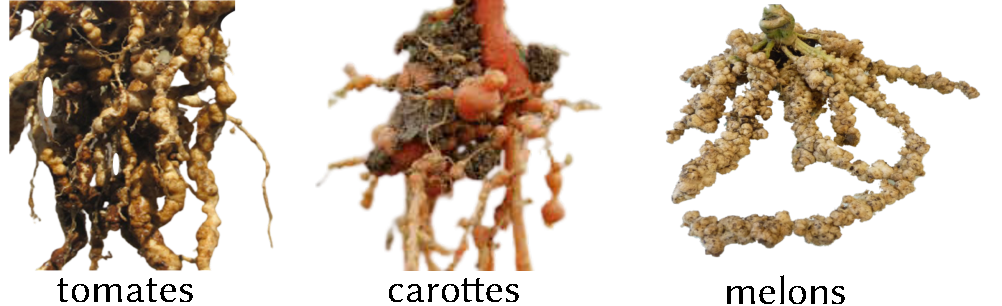
\includegraphics[width=0.7\linewidth]{galls.pdf}  

  \end{center}

\item<2> Dépérissement des parties aériennes
\item<2> Mort de  la plante (en cas de fortes infestations)  
  \hspace{-5mm}
  \begin{center}
      \begin{tikzpicture}
\visible<1>{\node  (img1){  \includegraphics<1>[width=0.5\linewidth]{degats2.pdf}};}
\visible<2>{\node (img1.south) {\includegraphics<2>[width=0.5\linewidth]{degats2.pdf}};}
 \end{tikzpicture} 

  \end{center}
 
   \end{itemize}}


\end{frame}


\subsubsection{Méthodes de lutte}


\begin{frame}[fragile]{Méthodes de lutte}

%\setbeamercovered{transparent}%
\setbeamercovered{invisible}
\vspace{-0.1cm}

\begin{columns}
 \begin{column}{.8\textwidth}
 \hspace{5mm} {\normalsize Lutte chimique:} 
  {\small          \begin{itemize}[leftmargin=1.22cm]
\item Contrôle longtemps basé sur l'usage  des pesticides 
\item La plupart de ces produits ont été bannis ou restreints \\(Directive UE 2007 \& Plan Ecophyto 2025)

            \end{itemize}}
 \end{column}

 \begin{column}{.31\textwidth}
 \hspace{6.5mm} {\small Pesticides}
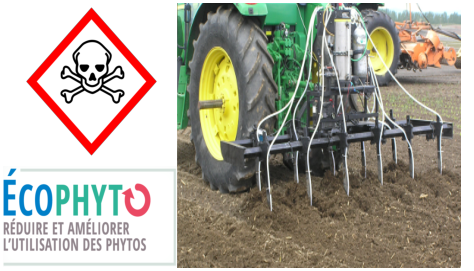
\includegraphics[width=0.75\linewidth]{Lutte_chimique}    
 \end{column}
\end{columns}
\pause

\begin{columns}
 \begin{column}{.8\textwidth}
\hspace{5mm}
{\normalsize Lutte physique : solarisation, désinfection vapeur  }
   { \small        \begin{itemize}[leftmargin=1.22cm]
\item Efficacité assez variable

            \end{itemize}}
 \end{column}

 \begin{column}{.3\textwidth}
\hspace{6mm} {\small Solarisation}

   \begin{tikzpicture}                 
            \visible<1-4>{\node[opacity=0.1] (img2) {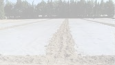
\includegraphics[width=.75\linewidth]{solarisation-transparency.pdf}};}
            \visible<2-4>{\node (img2)  {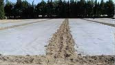
\includegraphics[width=0.75\linewidth]{solarisation.pdf}};}
         \end{tikzpicture}
 \end{column}
\end{columns}
\pause
\begin{columns}
 \begin{column}{.8\textwidth}
\hspace{5mm}
{\normalsize \begin{tabular}[t]{@{}l@{}} Lutte biologique : bactéries (Flocter$_{\mbox{\scriptsize{\textregistered}}}$ Bayer), \\
biopesticides issus de champignons \end{tabular}}
 {\small           \begin{itemize}[leftmargin=1.22cm]
\item Peu efficace

            \end{itemize}
} 
 \end{column}

 \begin{column}{.3\textwidth}
\hspace{6mm} {\small Bactéries}
   \begin{tikzpicture}                 
            \visible<1-4>{\node[opacity=0.3] (img3) {
\includegraphics[width=0.75\linewidth]{bac-transparency.pdf}};}
            \visible<3-4>{\node (img3)  {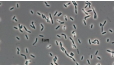
\includegraphics[width=0.75\linewidth]{bac.pdf}};}
         \end{tikzpicture} 
 \end{column}
\end{columns}

\pause
\begin{columns}
 \begin{column}{.8\textwidth}
 \hspace{5mm} 
{\normalsize \alert{\bf Résistance variétale} :}
{ \small
            \begin{itemize}[leftmargin=1.22cm]
\item  Efficace et respectueux de l'environnement
\item Peu de gènes majeurs (R) (exemple 
 \textit{Mi-1})
            \end{itemize}
 }\end{column}

 \begin{column}{.3\textwidth}
\hspace{6mm} { \small gène \textit{Mi}}\\
    \begin{tikzpicture}                 
            \visible<1-4>{\node[opacity=0.3] (img4) {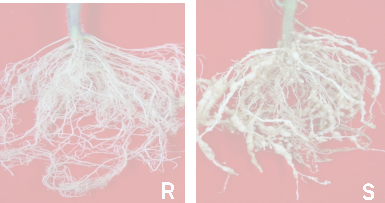
\includegraphics[width=0.75\linewidth]{root-transparency.pdf}};}
            \visible<4>{\node (img4)  {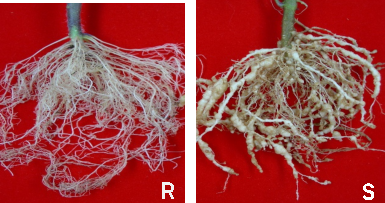
\includegraphics[width=0.75\linewidth]{root.pdf}};}
         \end{tikzpicture} 
 \end{column}
\end{columns}        
\end{frame}




\begin{frame}{La résistance qualitative}

	            \begin{itemize}[itemsep=10pt]
\item résistance totale $\Rightarrow$ engendre une absence de maladie 
\item  modèle gène pour gène (implication d'un gène R)  \textcolor{shadecolor}{\small [Flor, 1971]} 
            \end{itemize}
	
		\begin{center}

  \begin{tabular}{ccc}
    \hline
             & Plante résistante (R) & Plante sensible (S) \\
    \hline  
 \begin{tabular}[b]{@{}l@{}}Pathogène \\ avirulent 
  (\textit{Avr})
\end{tabular} &      		
			\includegraphics<1>[width=0.1\linewidth]{pasmalade}	
			\textcolor{vertmoyen}{saine}
			 & 	
			\includegraphics<1>[width=0.1\linewidth]{malade}	
			\textcolor{red}{infestation}
			 \\			    
 		
	\hspace{-3mm}	\begin{tabular}[b]{@{}l@{}}Pathogène \\ virulent 
  (\textit{Vir})
\end{tabular} & 		
	\hspace{-7mm}		\includegraphics<1>[width=0.1\linewidth]{malade}	
			\textcolor{red}{infestation}            &  		
			\includegraphics<1>[width=0.1\linewidth]{malade}	
			\textcolor{red}{infestation}
			       \\
    \hline
  \end{tabular}\\[0.5mm]
%        \begin{minipage}[c]{ 0.85 \linewidth}\small  Modèle d’interaction gène-pour-gène, 
%		           qui stipule qu'un gène 
%	     	       avirulent (\textit{Avr}) chez l’agent pathogène est identifié
%		           par un gène majeur de résistance  chez la plante \textcolor{shadecolor}{\small [Flor, 1971]} 
%        \end{minipage}  
	\end{center}
	

\end{frame}





\begin{frame}{Contournement}

\medskip
%
% \begin{alertblock}{Définition}
%
% On parle de contournement de la résistance lorsque tout ou partie de la population d'agents pathogènes s'est adaptée à la résistance et peut dès lors se développer comme s’il s’agissait de plantes sensibles
%\texttt{exampleblock}
%\end{alertblock}
		
\includegraphics[height=0.05\textheight]{danger}
	Déploiement des résistances $\Rightarrow$ sélection de génotypes
	virulents 
	\vfill
\begin{center}
		\includegraphics[width=.5\linewidth]{resitance-com}
\end{center}
	\vfill
	            \begin{itemize}[itemsep=10pt]
\item Exemple, le contournement du gène \textit{Mi} de la tomate \textcolor{shadecolor}{\small[Castagnone \textit{et al.,} 2002]}
\begin{center}
		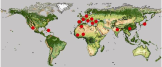
\includegraphics[height=0.4\textheight]{contournement-Mi}
\end{center}
          \end{itemize}
 \centering
 {\large \textcolor{red}{$\bullet$}} races de  \textit{meloidogyne} virulentes vis à vis du gène \textit{Mi}
\end{frame}


\begin{frame}{Coûts de virulence}
\setbeamercovered{invisible}
%	
%		
\includegraphics[height=0.05\textheight]{danger}
%	Déploiement des résistances $\Rightarrow$ sélection de génotypes
%	virulents 
	-\vspace{-5mm}
 \begin{beamercolorbox}[sep=5pt,rounded=true]{lightbox}
   
	\centering      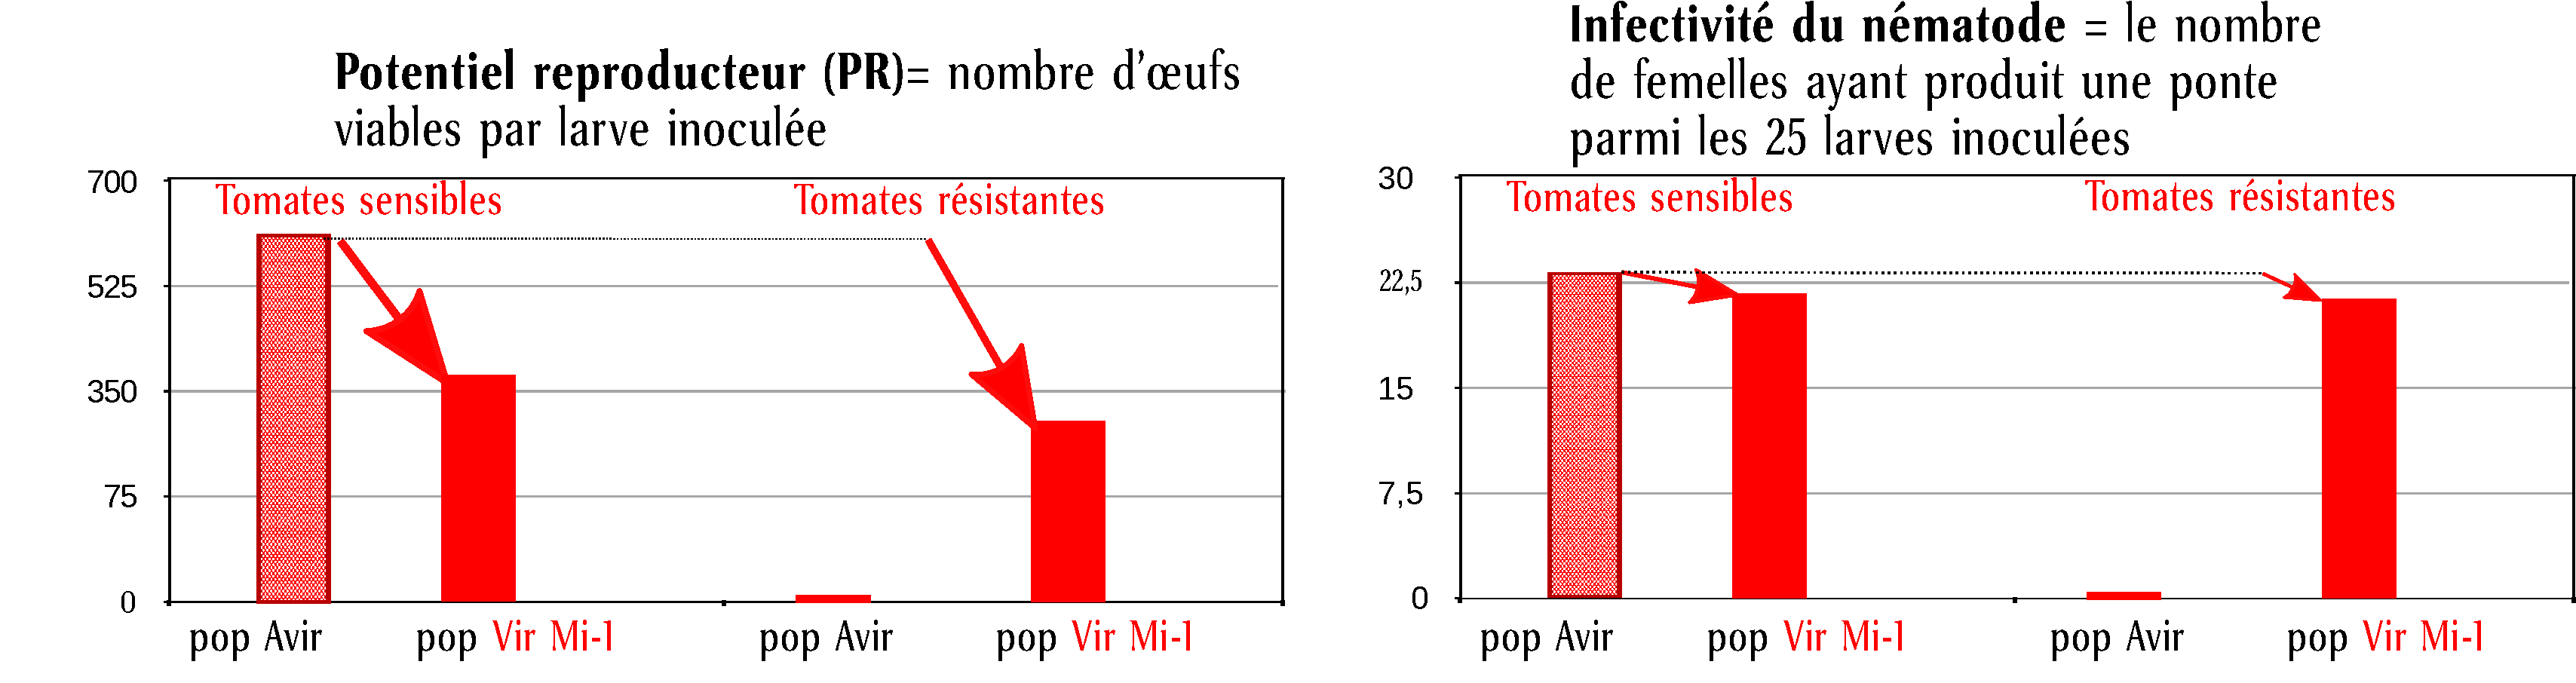
\includegraphics[width=1\linewidth]{cost-reproduction-infect.pdf}
%	\centering      \includegraphics<2>[width=.8\linewidth]{cost-infectivite} 
	
	
	\textcolor{shadecolor}{\small [Castagnone-sereno \textit{et al.}, 2007]	}
	
 \end{beamercolorbox}	
   \pause
  \small
 \begin{itemize}[itemsep=0mm]
  \item Plantes résistantes diminuent la population d'avirulents
\item Virulents sélectionnés sur plantes résistantes, mais contre-sélectionnés sur sensibles
\item  Combiner plantes résistantes \& sensibles pour diminuer la montée en fréquence des virulents
  \end{itemize}
\end{frame}


\begin{frame}{La stratégie de déploiement à l'étude}

%{\centering(justification de la recherche) } 
\setbeamercovered{invisible}
\begin{itemize}[itemsep=5mm]
\item Stratégies entre plantes résistantes et sensibles  existantes :
\end{itemize}

 \begin{center}
    \includegraphics<1>[width=1\linewidth]{strategies1.pdf}
    
  \includegraphics<2>[width=1\linewidth]{strategies2.pdf}
  
    \includegraphics<3>[width=1\linewidth]{strategies3.pdf}
  \end{center}
\uncover<3->{
\begin{outline}
\begin{itemize}[itemsep=5mm]
\item \textbf{Nématodes à galles peu mobiles }  $\Rightarrow$ \textbf{\textcolor{myvert}{rotations}}


\end{itemize}
\end{outline}
\par\bigskip
 

}

\end{frame}








\subsection{Objectifs}


\begin{frame}{Objectifs}

L’objectif principal de cette thèse est 

	\begin{center}\mbox{}
		\begin{beamercolorbox}[wd=.8\textwidth,sep=1ex,rounded=true]{darkbox}	
d’identifier des stratégies de déploiement de gènes R efficaces et
durables pour lutter contre les NG en culture maraîchère.
		\end{beamercolorbox}
	\end{center}\pause  
	pour ce faire
			\begin{enumerate}[itemsep=15pt]
	      \item la construction d'un modèle multi-saison 
       \item  la \textbf{calibration} du modèle sur des données de la littérature et nos données expérimentales 
         \item la recherche de \textbf{stratégies optimales de déploiement} en terme d'efficacité d'un gène R
          \item l’évaluation de la \textbf{robustesse} de ces stratégies
 	
	\end{enumerate}	
\end{frame}









\section[Modèle]{Description du modèle}


\begin{frame}{Notre approche de modélisation}
\begin{center}
  \vspace{3mm}
Cadre : modèles épidémiologiques type SIR \textcolor{shadecolor}{{\small[Kermack \& McKendrick (1927)]}}
   \begin{block}{ Nos hypothèses}
       \begin{itemize}[itemsep=10pt]
\item Échelle  $\rightarrow$	une plante 
\item Prise en compte de certaines particularités liées à la biologie du nématode
{\small\begin{itemize}[itemsep=10pt, label=$\rightarrow$]
\item Latence
\item Forme libre
\item Saisonnalité des systèmes de cultures : temps  continu (phase épidémique) et phénomènes discrets (survie) \textcolor{shadecolor}{{\small[Mailleret et \textit{al.,} 2012]}} \end{itemize}}
\item  Introduction résistance et  virulents
       \end{itemize}   
       \end{block} 

\end{center}

           \end{frame}
\subsection{Interaction plante  -- nématode}


\begin{frame}{Modèle interaction plante / nématode}
\setbeamercovered{invisible}
  \begin{center}
    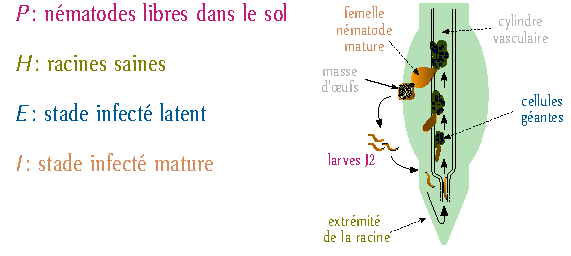
\includegraphics[width=.8\linewidth]{fig1V2.pdf}
  \end{center}
    \begin{columns}
      \hspace{5mm}
 \begin{column}{.5\textwidth}

	   \includegraphics<1>[width=1\linewidth]{mod0.pdf}
	    
	   \includegraphics<2>[width=1\linewidth]{mod1.pdf}
	    
	   \includegraphics<3>[width=1\linewidth]{mod2.pdf}
	   
	   \includegraphics<4>[width=1\linewidth]{mod3.pdf}
	     
	   \includegraphics<5>[width=1\linewidth]{mod4.pdf}
	    
	   \includegraphics<6>[width=1\linewidth]{mod5.pdf}
	    
	   \includegraphics<7>[width=1\linewidth]{mod6.pdf}

 \end{column}

\hspace{-10mm}

 \begin{column}{.5\textwidth}
  \begin{equation*}
    \left\{
      \begin{aligned}
        \dot{P} &= \uncover<2->{ -\beta\,P\,H }  \uncover<4->{  +r\,I} \uncover<5->{ - \eta\,P  ,}&\\  
       	\dot{H} &=  \uncover<6->{  \mu\,x\,} \uncover<7->{ f(.)}
       \uncover<2->{ - \epsilon\,\beta\,P\,H ,}&\\
        \dot{E} &= \uncover<2->{\epsilon\,\beta\,P\,H}
       \uncover<3->{  - \lambda\,E ,}&\\
        \dot{I} &=\uncover<3->{  \lambda\,E } \uncover<5->{ - \alpha\,I.}&\\
        \end{aligned}
      \right.
    \end{equation*}
 \end{column}
\end{columns}
\vspace{-2mm}
 \hspace{65mm}  
  \onslide<7>{  \begin{tabular}[t]{@{}l@{}}
 avec $f(.)=  e^{-k\, \pi}$,  $\pi=\frac{I}{H+E+I}$ 
    \end{tabular}}
\end{frame}
%
%  \begin{equation*}
%    \left\{
%      \begin{aligned}
%        \dot{P} &= -\beta\,P\,H   - \eta\,P +r\,I
%        &\qquad&\text{$P$ : nématodes dans le sol  } \\      
%       	\dot{H} &=   \mu\,x\,f(.)
%        - \beta\,\epsilon\,P\,H &\qquad& \text{$H$ : racines saines sensibles}\\
%        \dot{E} &= \beta\,\epsilon\,P\,H
%        - \lambda\,E
%        &\qquad& \text{$E$ : racines infectées en latence}\\
%        \dot{I} &= \lambda\,E
%        - \alpha\,I
%        &\qquad& \text{$I$ : racines infectées}
%        \end{aligned}
%      \right.
%    \end{equation*}



\subsection[Interaction plante résistante nématode (Nv) (1/2)]{Interaction plante R/nématodes}

\begin{frame}{}
\setbeamercovered{invisible}
 \frametitle{Interaction plante R / nématode  \rlap{\raisebox{-\dp\strutbox}{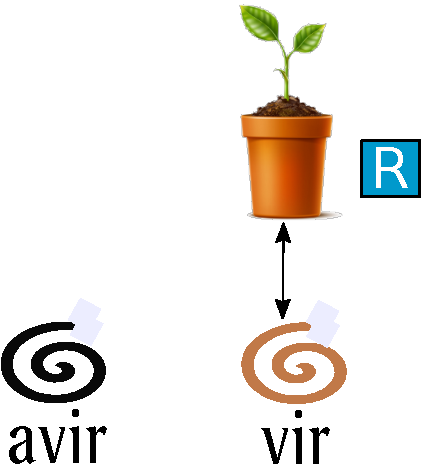
\includegraphics[height=2.5\baselineskip]{legPlantRnems.pdf}}}}
\begin{columns}
 \begin{column}{.5\textwidth}
 	\begin{center}
			\includegraphics<1>[width=0.8\linewidth]{diaPlantRnems0.pdf}
			
			\includegraphics<2>[width=0.8\linewidth]{diaPlantRnems1.pdf}
			
			\includegraphics<3>[width=0.8\linewidth]{diaPlantRnems2.pdf}
			\end{center}
			\hspace{3mm}

 \end{column}

 \begin{column}{.5\textwidth}
\small{
 \uncover<2-3>{\begin{equation*}
	 \left\{
		\begin{aligned}
		\dot{P_a} & =- \beta P_aH^R -\eta P_a ,&\\
		\dot{P_v} & =-\beta P_vH^R -\eta P_v   
		+ \uncover<3>{\textcolor{myorange}{(1-w_{r})}}r I_v,&\\
		\dot{H^R} &= \mu x f(.) 
		- \uncover<3>{\textcolor{myorange}{(1-w_{\beta})}} \epsilon_v^R \beta P_v H^R,& \\
		\dot{E_v} &=   \uncover<3>{\textcolor{myorange}{(1-w_{\beta})}} \epsilon_v^R \beta P_v H^R  - \lambda E_v, &\\
		\dot{I_v} & = \lambda E_v -\alpha I_v .&\\
		\end{aligned}
	\right.
\label{eq:ResistanceP-nemavir-nemvir}
\end{equation*}}}
 \end{column}
\end{columns}

%        \begin{minipage}[c]{ 1 \linewidth}\small  Modèle d’interaction gène pour gène (Flor, 1971) qui stipule qu’à
%chaque gène R d’une plante correspond un gène d’avirulence (gène Avr).
%        \end{minipage}
 
\hspace{15mm}

            \begin{itemize}        
 \item    \textcolor{myblue1}{Hôte  R}, nématodes avirulents (indice $_a$) et \textcolor{myor}{ virulents} (indice $_v$)
 \visible<2-3>{\item  Avirulents incapables d'infecter la plante \textcolor{myblue1}{R}}
 \visible<3>{\item Coût de \textcolor{myorange}{virulence} sur l'infectivité ($w_{\beta}$) et la reproduction ($w_r$)}
            \end{itemize}

\end{frame}


\subsection[Interaction plante résistante nématode (Nv) (1/2)]{Interaction plante S/nématodes}



\begin{frame}{}

\setbeamercovered{invisible}
 \frametitle{Interaction plante S / nématode  \rlap{\raisebox{-\dp\strutbox}{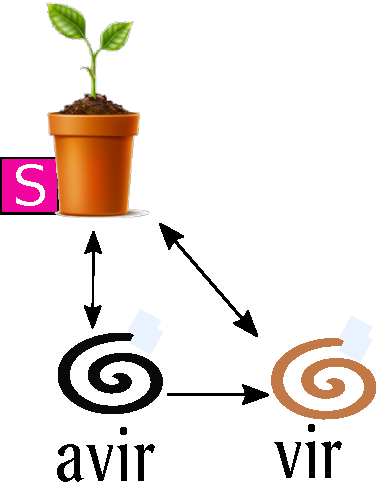
\includegraphics[height=2.5\baselineskip]{legPlantSnems1.pdf}}}}
\begin{columns}
 \begin{column}{.5\textwidth}
 	\begin{center}
 				\includegraphics<1>[width=0.8\linewidth]{diaplantSnems0.pdf}
 				
			\includegraphics<2>[width=0.8\linewidth]{diaplantSnems1.pdf}
			\end{center}
 
 \end{column}
 
 \hspace{-5mm}
 \begin{column}{.5\textwidth}
\small{\begin{equation*}
	\left\{
		\begin{aligned}
		\dot{P_a} & =- \beta P_aH^S -\eta P_a + \uncover<2->{\textcolor{red}{(1-\delta)}}r I_a,&\\
		\dot{P_v} & =-\beta P_vH^S -\eta P_v  + (1-w_{r})r I_v + \uncover<2->{\textcolor{red}{\delta}} r I_a &\\
		\dot{H^S} &= \mu x f(.)  -\epsilon_a^S
		\beta P_a H^S  -(1-w_{\beta}) \epsilon_v^S \beta P_v H^S,& \\
		\dot{E_a} &= \epsilon_a^S \beta P_a H^S  - \lambda E_a, &\\
		\dot{E_v} &=  (1-w_{\beta}) \epsilon_v^S \beta P_v H^S  - \lambda E_v, &\\
		\dot{I_a} & = \lambda E_a - \alpha I_a ,&\\
		\dot{I_v} & = \lambda E_v - \alpha I_v .&\\
		\end{aligned}
	\right.
	\label{eq:mod-sensible}
\end{equation*}}
 \end{column}

\end{columns}
            \begin{itemize}
 \item Avirulents et \textcolor{myor}{virulents}  peuvent infecter  \textcolor{mypink}{Hôte S}
\item Coût de virulence sur l'infectivité ($w_{\beta}$) et la reproduction ($w_r$)
  
 \uncover<2->{\item \textcolor{red}{Fraction $\delta$} d'avirulents $\rightarrow$ \textcolor{myor}{ virulents}} \\
 \end{itemize}   

\end{frame}

\subsection{Modèle multi-saison (complet)}
\begin{frame}{Modèle multi-saison}
	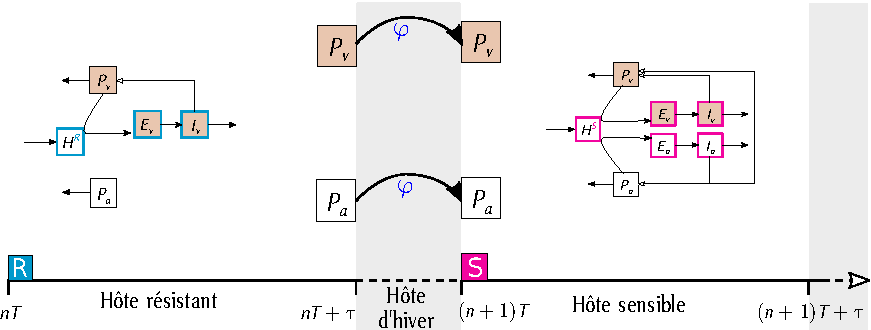
\includegraphics[width=\linewidth]{semi_discret_comp_NSbis.pdf}
	\par\bigskip
	\textcolor{blue}{Survie inter-saison} des nématodes en présence de culture d'hiver :
	\begin{equation*}
		\left\{
		 \begin{aligned}		  
		    P_v ((n+1)T) &= \textcolor{blue}{\varphi} P_v(nT + \tau)\\
		    P_a ((n+1)T) &= \textcolor{blue}{\varphi} P_a(nT + \tau)
		 \end{aligned}
		\right.
		\label{eq:intersaison-nemavir-nemvir}
	\end{equation*}

\end{frame}

\section{Calibration}
\subsection{Ajustement du modèle intra-saison}




\begin{frame}{Données}

\setbeamercovered{invisible}  
\medskip
\begin{itemize}[itemsep=15pt]
\item Toutes  les  valeurs de paramètres sont issues de la littérature sauf 3 :
	{\small
	\begin{itemize}[label=\ding{51},leftmargin=2cm]
	\item[$\rightarrow$] $\beta$ taux d'infection
	\item[$\rightarrow$] $k$ facteur de modulation de la croissance
	\item[$\rightarrow$] $x$ facteur de conversion
	\end{itemize}}
	
  
  \pause
\item 1 expérience, 5 valeurs de
densités initiales \textcolor{shadecolor}{\small[Ehwaeti \textit{et al.,} 1998]}:
	{\small
	\begin{itemize}[label=\ding{51},leftmargin=2cm]
	\item[$\rightarrow$] Densité finale de nématodes dans la plante à 42 et 135 jours
	\item[$\rightarrow$]  Biomasse racinaire à 42 et 135 jours
	\end{itemize}}
	
\item 1 nouvelle expérience (ISA 2018), 3 valeurs de
densités initiales : 
\end{itemize}

 \begin{columns}
 \begin{column}{.52\textwidth} 
	{\small
	\begin{itemize}[label=\ding{51},leftmargin=2cm]
	\item[$\rightarrow$] Densité finale de nématodes dans la plante à 35 jours
	\item[$\rightarrow$] Biomasse racinaire à 35 jours
	\end{itemize}}
 \end{column}

 \begin{column}{.55\textwidth} 

	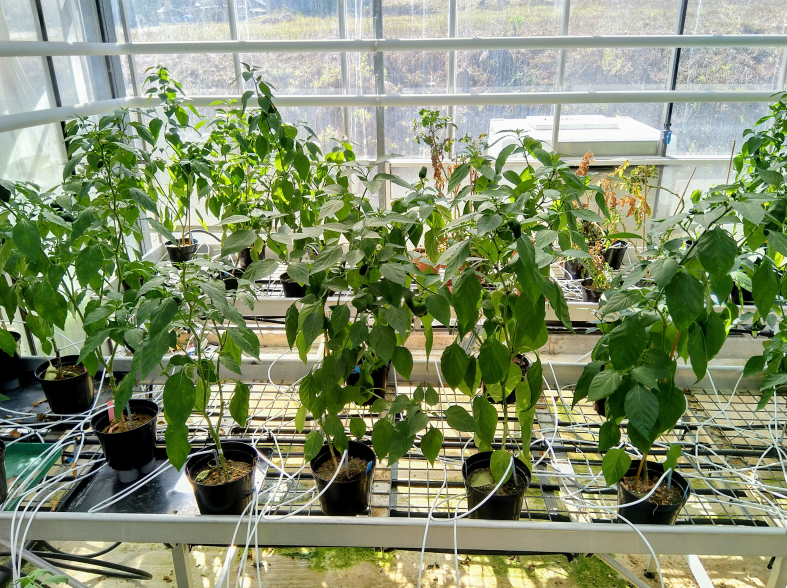
\includegraphics[width=0.45\linewidth]{expe.png}
 \end{column}
\end{columns}
\end{frame}











\begin{frame}{Calibration (Ehwaeti \textit{et al.,} (1998))}  

\setbeamercovered{invisible}   

\centering
		\includegraphics<1>[width=1\linewidth]{fig2V1.pdf}
		
		\includegraphics<2>[width=1\linewidth]{fig2V2.pdf}		

		\includegraphics<3>[width=1\linewidth]{fig2V3.pdf}

\vfill
\visible<2-3>{
	\begin{beamercolorbox}[sep=0.5mm,rounded=true]{lightbox}
	  	\ding{229}  \textbf{Bon ajustement} du modèle\\
	  	\onslide<3>{\ding{229} \textbf{Validation} du modèle  }
  \end{beamercolorbox}}
\end{frame}

\begin{frame}{Calibration (nos données)}   
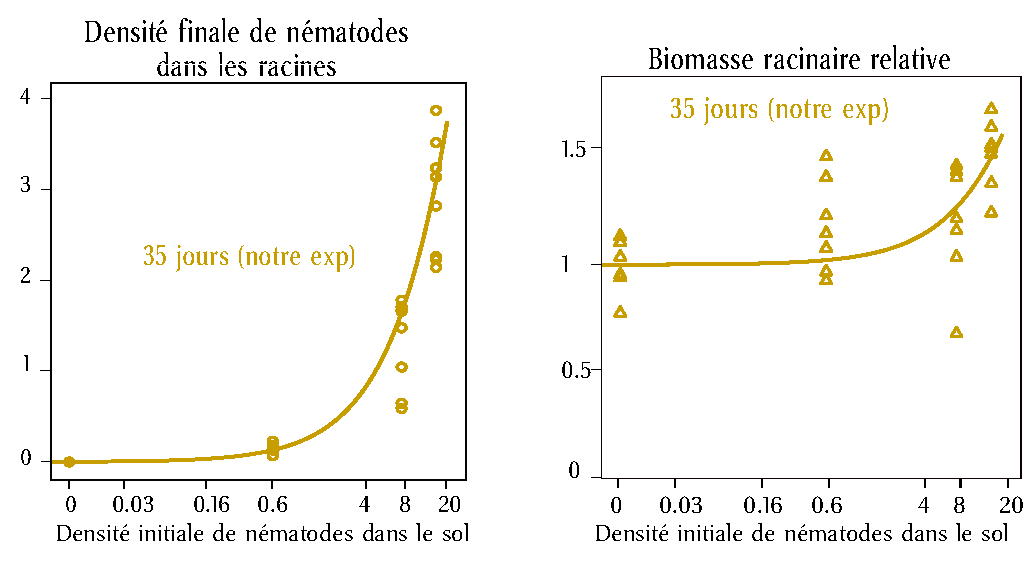
\includegraphics[width=1\linewidth]{fit_exp.pdf}

	\begin{beamercolorbox}[sep=0.5mm,rounded=true]{lightbox}
	  	
\ding{229} \textbf{Bon ajustement} du modèle à nos données
  \end{beamercolorbox}

\end{frame}





\begin{frame}{Conclusions}
 \begin{beamercolorbox}[sep=1mm,rounded=true]{lightbox}
  \begin{itemize}[itemsep=6mm]
 \item \textbf{Bon ajustement} du modèle à des jeux de  données issues  d'expériences \\différentes     $\Rightarrow$  \textbf{modèle  très adaptable} 
   \item Paramètres ajustés très similaires entre les deux ajustements $\Rightarrow$ bonne confiance  en les valeurs  de paramètres estimés (non présenté)

  \end{itemize}
 \end{beamercolorbox}
\end{frame}


\section[Rotations]{Stratégies de déploiement de la résistance}
\subsection{Définition des stratégies et critère d'optimisation}



 
 \begin{frame}{Définition  des stratégies}
 
  \begin{minipage}[t]{0.49\linewidth}
    \begin{block}{Stratégies pures}
      \medskip
      \begin{tabular}{@{}l@{~}l@{}l}
        plantes résistantes &\Rb\Rb\Rb\Rb\Rb... \\[2mm]
        plantes sensibles &\Sb\Sb\Sb\Sb\Sb... \\
        \mbox{}
      \end{tabular}
    \end{block}
  \end{minipage}
  \hfill
     \begin{minipage}[t]{0.44\linewidth}
    \begin{block}{Rotations périodiques}
      \medskip
      \textcolor{myblue1}{$y$} saisons  \Rb\ \& \textcolor{mypink}{$x$} saisons
      \Sb... \\[2mm]
      Exemple :  \textcolor{myblue1}{$y=1$} \&  \textcolor{mypink}{$x=2$} \\[1mm]
      \Rb\Sb\Sb\Rb\Sb\Sb\Rb\Sb\Sb\Rb\Sb...
    \end{block}
  \end{minipage}
\hspace{-4mm}
   \begin{minipage}[t]{0.44\linewidth}
    \begin{block}{Rotations sans contraintes}
      \medskip
      \Rb\Sb\Sb\Sb\Rb\Rb\Rb\Sb\Sb\Rb\Sb...
    \end{block}
  \end{minipage}
 \end{frame}
 
 
 
\begin{frame}{Simulations}
\centering
    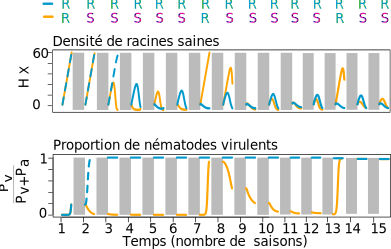
\includegraphics[width=0.8\linewidth]{simulation}
      \begin{beamercolorbox}[sep=0.5mm,rounded=true]{lightbox}
   \begin{tabular}[t]{@{}l@{}}
   \ding{229}Fixation rapide des virulents (dès la deuxième année)
   \end{tabular}\\
  \ding{229}En alternant la résistance par la stratégie 1R+5S  $\rightarrow$ alternance des pressions sélectives\\
   
\end{beamercolorbox}
\end{frame}


\begin{frame}{Optimisation}
   \begin{block}{Critère à maximiser}
     \begin{itemize}
     \item Proxy de rendement
       \begin{itemize}
       
       \item[$\rightarrow$] \textbf{« Rendement » saisonnier moyen} (aire sous la courbe de densité des racines saines pour
un nombre donné de saisons $n$) : \\
       \begin{equation*}
  \overline{HRD}=\frac{1}{n} \sum_{i=1}^{n} \int_{i^{\text{ème}}\text{ saison}} H^{X}(t) dt
  \label{hr}
\end{equation*}
       \end{itemize}
              \item Similaire à la durée de la surface foliaire saine ($HAD$) \textcolor{shadecolor}{{\small[Van den Bosch \& Gilligan, 2003; Papaïx
et \textit{al.,} 2018]}}
     \item Stratégie optimale = maximisation de l'$\overline{HRD}$
     \end{itemize}
   \end{block}
   
   \begin{block}{Méthode}
        \begin{itemize}[itemsep=6pt]
     \item Horizon temporel 2 à 30 ans

     \item Rotation sans contrainte optimale : algorithme génétique
          
     \item Rotation périodique optimale :  méthode exhaustive  
     
       \end{itemize}
  \end{block}
   
 \end{frame}

\subsection{Stratégies optimales}
\subsubsection{Paramètres de références}
\subsubsection{Caractéristiques de la résistance}
\subsubsection{Scénarios épidémiologiques}
\subsubsection{La robustesse}


\begin{frame}{Recherche de la stratégie périodique optimale}

\setbeamercovered{invisible}
  \centering
      \includegraphics<1>[width=0.7\linewidth]{fig3bis1.pdf}
      
            \includegraphics<2>[width=0.7\linewidth]{fig3bis2.pdf}

    \includegraphics<3>[width=0.7\linewidth]{fig3bis3.pdf} 
       
  \vfill



\onslide<3>{  \begin{beamercolorbox}[sep=1mm,rounded=true]{lightbox}

  \ding{229}  \textcolor{myorange}{ Rotation périodique optimale} >  stratégie \textcolor{myblue1}{100 \% R} et \textcolor{mypink}{100 \% S}

 
 \end{beamercolorbox}}
\end{frame}

%\begin{frame}{Résultats : stratégie optimale (Rendement)}
%  \vfill
%  \includegraphics[width=\linewidth]{triangle102030ans}
%  \vfill\vfill
%  \pause
%  \begin{beamercolorbox}[sep=1mm,rounded=true]{lightbox}
%  \ding{229}
%  \begin{tabular}[t]{@{}l@{}}
%    \textbf{Rotation optimale} meilleure que les stratégies pures \\
%    1 seule saison \Rb\ par période
%  \end{tabular}
%\end{beamercolorbox}
%\end{frame}



\begin{frame}{ Stratégies de rotation périodique optimale}

\setbeamercovered{invisible}

\begin{center}
\begin{tikzpicture}

    \only<1->{
        \node[anchor=south west,inner sep=0] (B) at (0,0) {\includegraphics<1>[width=0.55\linewidth]{fig4V1} };
    }

    \only<2->{
        \node[anchor=south west,inner sep=0] (C) at (0,0) {\includegraphics<2>[width=0.55\linewidth]{fig4V2} };  }

    \only<3->{
        \node[anchor=south west,inner sep=0] (C) at (0,0) {\includegraphics<3>[width=0.55\linewidth]{fig4V3} };  }
\end{tikzpicture}
\end{center}

    \begin{beamercolorbox}[sep=0.5mm,rounded=true]{lightbox}
 \ding{229} 
    \textbf{Efficacité des stratégies} chute rapidement avec
horizon temporel \\

 \onslide<2->{

 \ding{229}  Gain relatif $\nearrow$ avec horizon temporel}
\end{beamercolorbox}

\end{frame}






\begin{frame}{Conclusions}
 \begin{beamercolorbox}[sep=1mm,rounded=true]{lightbox}
  \begin{itemize}[itemsep=3mm]
  	
   \item Stratégies de \textbf{rotations périodiques}  >  stratégie pures résistantes
  
   \item Quand la résistance est contournée \textbf{ la stratégie optimale} est caractérisée par de \textbf{faibles ratios de plantes résistantes} (non présenté)
    \item  \textbf{Rotation périodique optimale} quasiment \textbf{l'optimum} pour assurer les meilleurs rendements
  \end{itemize}
\end{beamercolorbox}

\end{frame}

\section{Robustesse}

\begin{frame}{Analyse de sensibilité}


\begin{columns}

 \begin{column}{.5\textwidth}
 
\begin{block}{Objectif et méthode}
\begin{itemize}[itemsep=10pt]

\item Trouver les paramètres les plus influents sur le $\overline{HRD}$ (stratégie optimale 1R+5S sur 15 saisons) 
\item Paramètres : $\pm{30\%}$ de la valeur de référence \\(plan factoriel fractionnaire) 
\item Indices de sensibilité (Anova)

\end{itemize}

\end{block}
\end{column}

 \begin{column}{.5\textwidth}

 \begin{center}

    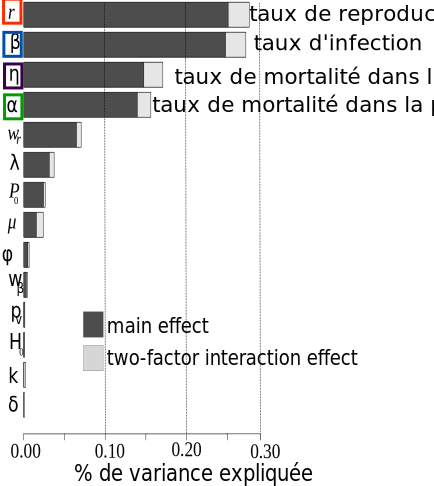
\includegraphics[width=1\linewidth]{ans}

 \end{center}


\end{column}
\end{columns}
        
\end{frame}

\begin{frame}{Scénarios épidémiologiques }

%\begin{outline}
%\begin{itemize}[itemsep=15pt]
%
%\item À partir des 4  paramètres épidémiologiques les plus influents,  3 scénarios épidémiologique :
% {\small\begin{itemize}[label=$\rightarrow$]
%\item \textcolor{myblue4}{Intermédiaire}
%\item \textcolor{mypink2}{Élevé}
%\item \textcolor{mypurple2}{Extrême}
%\end{itemize}}
%        
%\item Des variations de $\pm{10\%}$,  $\pm{20\%}$,  $\pm{30\%}$ au sein des 3 scénarios pour étudier la robustesse des stratégies :
% {\small
% \begin{itemize}[label=$\rightarrow$]
%\item savoir si \textbf{le gain relatif} issu de la stratégie  se maintient
%face à ces variations de paramètres
%\end{itemize} 
%}
%\end{itemize}
%\end{outline}


\begin{block}{Définition des scénarios}
     \begin{itemize}
     \item À partir des 4  paramètres épidémiologiques les plus influents,  3 scénarios épidémiologiques :
 {\small \begin{itemize}[label=$\rightarrow$]
\item \textcolor{myblue4}{Référence}
\item \textcolor{mypink2}{Élevé} (taux de reproduction et d'infection plus élevés)
\item \textcolor{mypurple2}{Extrême}  (taux de mortalité plus faibles)
\end{itemize}}
\end{itemize}
   \end{block}
   
   \begin{block}{Robustesse}
Pour chaque scénario :
     \begin{itemize}
     \item Déterminer la rotation périodique optimale
     \item En appliquant cette rotation, déterminer si \textbf{le gain relatif} se maintient
face à des variations de paramètres
\end{itemize}
   \end{block}
   

\end{frame}

%
%\begin{frame}{Scénarios épidémiologiques }
%
%\begin{outline}
%\begin{itemize}[itemsep=15pt]
%
%\item $\pm{30\%}$ sur ces paramètres, 4 scénarios   
%     \vspace{5mm}
%       \begin{tabular}{lccccc}
%    \hline
%    Scenario & $\beta$ & $r$     & $\alpha$ & $\eta$  \\
%    \hline
%    faible      & $-30\%$ & $-30\%$ & $+30\%$  & $+30\%$ \\
%    intermédiaire   & --      & --      & --       &  --     \\
%    élevé     & $+30\%$ & $+30\%$ & --       &  --     \\
%    Extrême  & $+30\%$ & $+30\%$ & $-30\%$  & $-30\%$ \\
%    \hline
%  \end{tabular}
%        
%\item $\pm{10\%}$,  $\pm{20\%}$,  $\pm{30\%}$ sur 3 scénarios   
%\end{itemize}
%\end{outline}
%
%
%\end{frame}

\begin{frame}{Robustesse}
\setbeamercovered{invisible}
  \begin{center}
    \includegraphics<1>[width=0.6\linewidth]{fig7bis1}
    
    \includegraphics<2>[width=0.6\linewidth]{fig7bis2}
  \end{center}

  \vspace{-.1cm}
  \uncover<2->{    \begin{beamercolorbox}[sep=0.5mm,rounded=true]{lightbox}
   \begin{tabular}[t]{@{}l@{}}
 \ding{229} Rotation périodique optimale presque toujours plus efficace que  100\%R  

   \end{tabular}
   
\end{beamercolorbox}}
\end{frame}



\begin{frame}{Conclusions}
 \begin{beamercolorbox}[sep=1mm,rounded=true]{lightbox}
  \begin{itemize}[itemsep=3mm]

  \item Paramètres épidémiologiques : les plus influents, valeurs souvent incertaines $\rightarrow$ scénarios
  
  \item \textbf{Efficacité} de la rotation  optimale  \textbf{même avec incertitude} sur valeur des paramètres, surtout pour des \textbf{situations épidémiologies élevées et extrêmes}
 
  \end{itemize}
\end{beamercolorbox}


\end{frame}

\section[Caract. R]{Caractéristiques de la résistance}

\begin{frame}{Caractéristiques de la résistance}

\setbeamercovered{invisible}

	 %Deux types de caractéristiques:   
			\begin{enumerate}[itemsep=10pt]
			       \item  Coûts de virulence  
	      \item Mode d'action de la réponse  de la plante résistante (précoce/tardive)



			\end{enumerate}
Exemple chez le piment :\\

 \begin{columns}
 \begin{column}{.52\textwidth} 
\centering

  Résistance précoce

 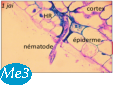
\includegraphics[width =0.5\textwidth]{Me3}\\
 $\downarrow$\\
 	facilement contournable
 \end{column}
 \begin{column}{.55\textwidth} 

\centering
 Résistance tardive
 
 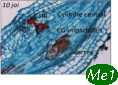
\includegraphics[width =0.5\textwidth]{Me1}\\
 	$\downarrow$\\
 	difficilement contournable
 \end{column}
\end{columns}
\begin{center}
\alert{Comment expliquer ces différences ?}

\end{center}
\end{frame}

\subsection{Influence  des coûts de virulence}
\begin{frame}{ Influence des coûts de virulence}

\setbeamercovered{invisible}
\centering
    \includegraphics<1>[width=0.5\linewidth]{fig_fitness_cost0}   

   \includegraphics<2>[width=0.5\linewidth]{fig_fitness_cost1}

   \includegraphics<3>[width=0.5\linewidth]{fig_fitness_cost2}
   \vfill
\visible<2-3>{
    \begin{beamercolorbox}[sep=0.5mm,rounded=true]{lightbox}
\uncover<2->{\begin{tabular}[t]{@{}l@{}} \ding{229} Coûts élevés  : pas de contournement \end{tabular}\\
\ding{229} Coûts faibles  : peu de contre-sélection des virulents sur plante sensible
}\\
\uncover<3->{\ding{229} \textcolor{red}{Données tomate \textit{Mi}} \textcolor{shadecolor}{\small[Castagnone \textit{et al.,} 2002]} : gain relatif >30 \% }
\end{beamercolorbox} }


\end{frame}

\begin{frame}{Influence des coûts de virulence}

\setbeamercovered{invisible}
\centering
   \includegraphics<1>[width=0.55\linewidth]{fig_gain3}   

   \includegraphics<2>[width=0.55\linewidth]{fig_gain4}

   \includegraphics<3>[width=0.55\linewidth]{fig_gain6}

   

\vspace{-0.1mm}

%
%\uncover<5->{\ding{229} Courbes de niveaux de w : superposition avec les courbes de niveaux du gain relatif}


   \small
\visible<3>{
    \begin{beamercolorbox}[sep=0.1mm,rounded=true]{lightbox} 
  \onslide<3>{
  \begin{equation*}
R_{0,v} = \varphi \exp\left(\beta\left( \frac{ \textcolor{red}{(1-(w_{\beta}+w_r- w_{\beta} w_r))}\epsilon_v r}{\alpha}-1\right) \left( H_0 \tau+\frac{\mu x \tau^2}{2}\right)-\eta \tau\right). \label{R0v}
\end{equation*}
}
 \onslide<3>{\ding{229} Mieux vaut un fort coût de virulence que deux coûts de virulence intermédiaires }
\end{beamercolorbox} }

\end{frame}



\subsection{Comparaison gènes tardifs et précoces}

\begin{frame}{}
\setbeamercovered{invisible}
 \frametitle{2. Comparaison gènes tardifs et précoces}
\begin{columns}
 \begin{column}{.5\textwidth}
 \centering
 \textcolor{myblue1}{  R précoce} 
		%	\includegraphics<1>[width=0.8\linewidth]{resPrecoce0}
			
			\includegraphics<1>[width=0.8\linewidth]{resPrecoce1}
			
			\includegraphics<2>[width=0.8\linewidth]{resPrecoce2}
			
	

 \end{column}

 \begin{column}{.5\textwidth}
\centering
 \textcolor{mygreen}{  R tardive} 
	%		\includegraphics<1>[width=0.8\linewidth]{resTardive0}
			
		  \includegraphics<1>[width=0.8\linewidth]{resTardive1}
			
			\includegraphics<2>[width=0.8\linewidth]{resTardive2}
			
	
 \end{column}
\end{columns}

%        \begin{minipage}[c]{ 1 \linewidth}\small  Modèle d’interaction gène pour gène (Flor, 1971) qui stipule qu’à
%chaque gène R d’une plante correspond un gène d’avirulence (gène Avr).
%        \end{minipage}
 \vfill
            \begin{itemize}       

%  \visible<2-3>{\item Coût de \textcolor{orange}{virulence} sur l'infectivité (précoce $w_{\beta}$ ou tardive $w_{\lambda}$) et la reproduction ($w_r$)}

\visible<1-2>{
\item \textcolor{mygreen}{  R tardive} : nématodes avirulents bloqués au bout d'un temps  \textcolor{myblue3}{$\frac{1}{\sigma}$} $\rightarrow$ fraction \textcolor{myblue3}{$\psi$} de racines infestées alors \textcolor{myblue3}{immunisées} \textcolor{myblue3}{G} 
}

            \end{itemize}

\end{frame}

\begin{frame}{2. Comparaison gènes R précoce et tardif}

\setbeamercovered{invisible}
\centering
    \includegraphics<1>[width=1\linewidth]{compar0.pdf}  
    
    \includegraphics<2>[width=1\linewidth]{compar1.pdf}   




    \begin{beamercolorbox}[sep=0.5mm,rounded=true]{lightbox}
 \begin{tabular}[t]{@{}l@{}}
\ding{229} Mêmes efficacités, mêmes rotations périodiques optimales (non montrées)
  \end{tabular}\\
\uncover<2->{\ding{229} Résultats identiques pour des coûts de virulence élevés}
\end{beamercolorbox} 
\end{frame}




%\invisible{$w_r$ and $w_{\beta}$ symétriques, contour plot gain concave, $w_r$ and $w_\beta$ interaction négative   }\\



%\section[Comparaison gène R]{Comparaison de la résistance précoce et tardive}
%\subsection{Rotations optimales avec gènes majeurs précoces ou tardifs}
%\subsection{Durabilité des gènes majeurs précoces et tardifs }
%%\subsection{Introduction d’un réservoir de plantes sensibles non cultivées} .
%\subsection{Comparaison de deux mesures de durabilité pour une résistance tardive }


\begin{frame}{Conclusions}
 \begin{beamercolorbox}[sep=1mm,rounded=true]{lightbox}
 \begin{itemize}[itemsep=3mm]
   
 \item \textbf{Pas d’impact des mécanismes seuls tardifs et précoces},
mieux vaut des coûts de virulence élevés pour éviter le contournement
 \end{itemize}
\end{beamercolorbox}


\end{frame}

\section{Conclusions générales}

\begin{frame}{Conclusions}
 \begin{beamercolorbox}[sep=1mm,rounded=true]{lightbox}
 \begin{itemize}[itemsep=3mm]
    
\setbeamercovered{invisible}
 \item \textbf{Modèle générique} pouvant s'adapter à différentes interactions plantes\\ nématodes
 \pause

 \item \textbf{Rotations} entre plantes résistantes et sensibles \textbf{plus efficaces} que \\ l'approche  conventionnelle 100\% R,  surtout quand :
    {\small \begin{itemize}
    \item Horizons longs 
    \item Coûts de virulence intermédiaires
    \item Niveaux épidémiologiques élevés et extrêmes
    \end{itemize}
   
}
 \pause
  \item Efficacité de la rotation  optimale  \textbf{maintenue même avec incertitude sur les valeurs  des paramètres} du modèle
 \pause 
  \item Favoriser les variétés résistantes sur la base des coûts de virulence induits, plus que sur leur mode d'action (mais lien possible entre mode d'action et coûts) 
 \end{itemize}
\end{beamercolorbox}

\end{frame}

\begin{frame}{Publication et conférences}

 \begin{beamercolorbox}[sep=1mm,rounded=true]{lightbox}

    
Publication :


\includegraphics[width =0.5\textwidth]{evol.png} \quad

 \begin{itemize}[itemsep=3mm]
 \item  Nilusmas \textit{et al.}, 2020, \textit{Evolutionary Applications} (volume 13, pages 2206-2221)
 \end{itemize}

Conférences :
 \begin{itemize}[itemsep=3mm]
 \item HORTIMODEL 2016, Avignon
 \item Ecology and Agriculture Summit for Young scientists 2017, CEBC Chizé
 \item ECMTB 2018, Lisbonne
 
 \end{itemize}
\end{beamercolorbox}


\end{frame}
%%
%\begin{frame}{Perspectives}
%
%  \begin{alertblock}{}
%    \begin{itemize}
%    \item Obtenir davantage de données saisonnières issues de parcelles  pour confronter nos résultats
%    \item Améliorer le critère de rendement en considérant la partie racinaire et végétale 
%    \end{itemize}
%
%    \begin{itemize}
%
%       
%      \item  Intégrer différentes architectures génétiques (alternance de gènes de résistance pyramidage de gènes de résistance vs gène unique)
%        \item Étudier la résistance dans le cas de l'utilisation d'une résistance partielle 
%      \item    Elargir la problématique à l’échelle des exploitations pour gérer le déploiement spatio-temporelle des résistances 
%     \end{itemize}
%  \end{alertblock}
%\end{frame}
%
%
%{
%\usebackgroundtemplate{%
%
%\tikz\node[opacity=1,inner sep=0] {\includegraphics[height=\paperheight,width=\paperwidth]{background.pdf}};}
\begin{frame}{Perspectives}
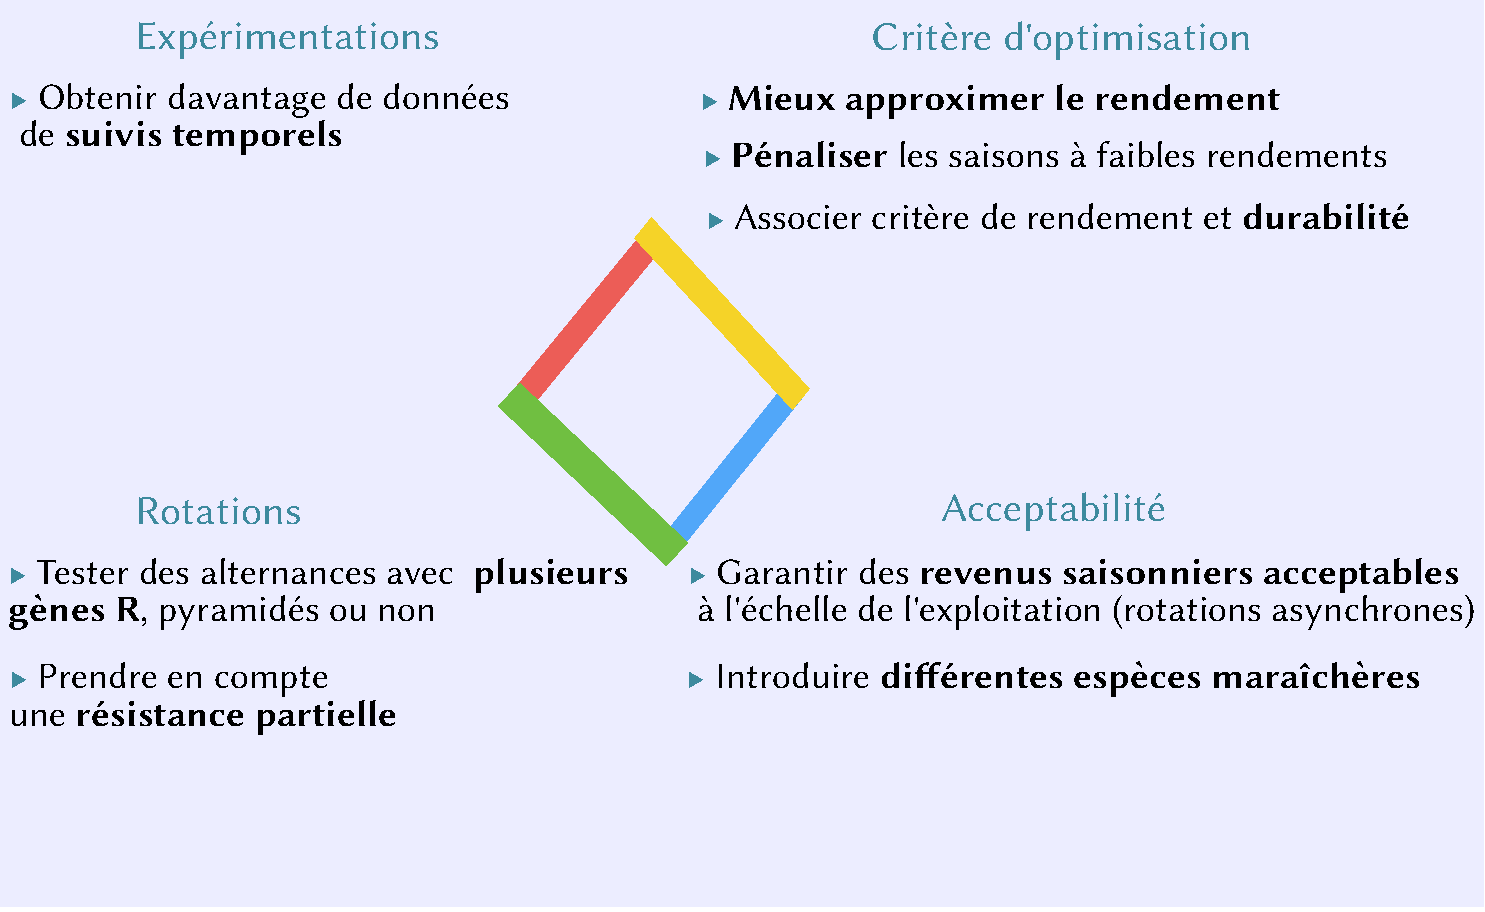
\includegraphics[width=1\linewidth]{perspectives}
%\begin{textblock*}{5cm}(10cm,7cm) % {block width} (coords)
%\shadowimage[width=2cm]{paysage.jpg} \quad
%\end{textblock*}
 \begin{textblock*}{5cm}(7cm,7.6cm) % {block width} (coords)
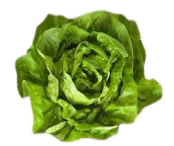
\includegraphics[width =0.1\textwidth]{laitue} \quad
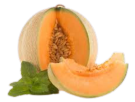
\includegraphics[width =0.15\textwidth]{melon} \quad
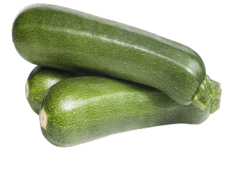
\includegraphics[width =0.15\textwidth]{courgette} 
\end{textblock*}
\begin{textblock*}{5cm}(10cm,7.2cm) % {block width} (coords)
\shadowimage[width=2cm]{piment.png} \quad
\end{textblock*}
 \begin{textblock*}{5cm}(2cm,3cm) % {block width} (coords)
\shadowimage[width=2cm]{expe} \quad
\end{textblock*}
\end{frame}



\begin{frame}[t]{}


\begin{textblock*}{5cm}(-0.4cm,2cm) % {block width} (coords)
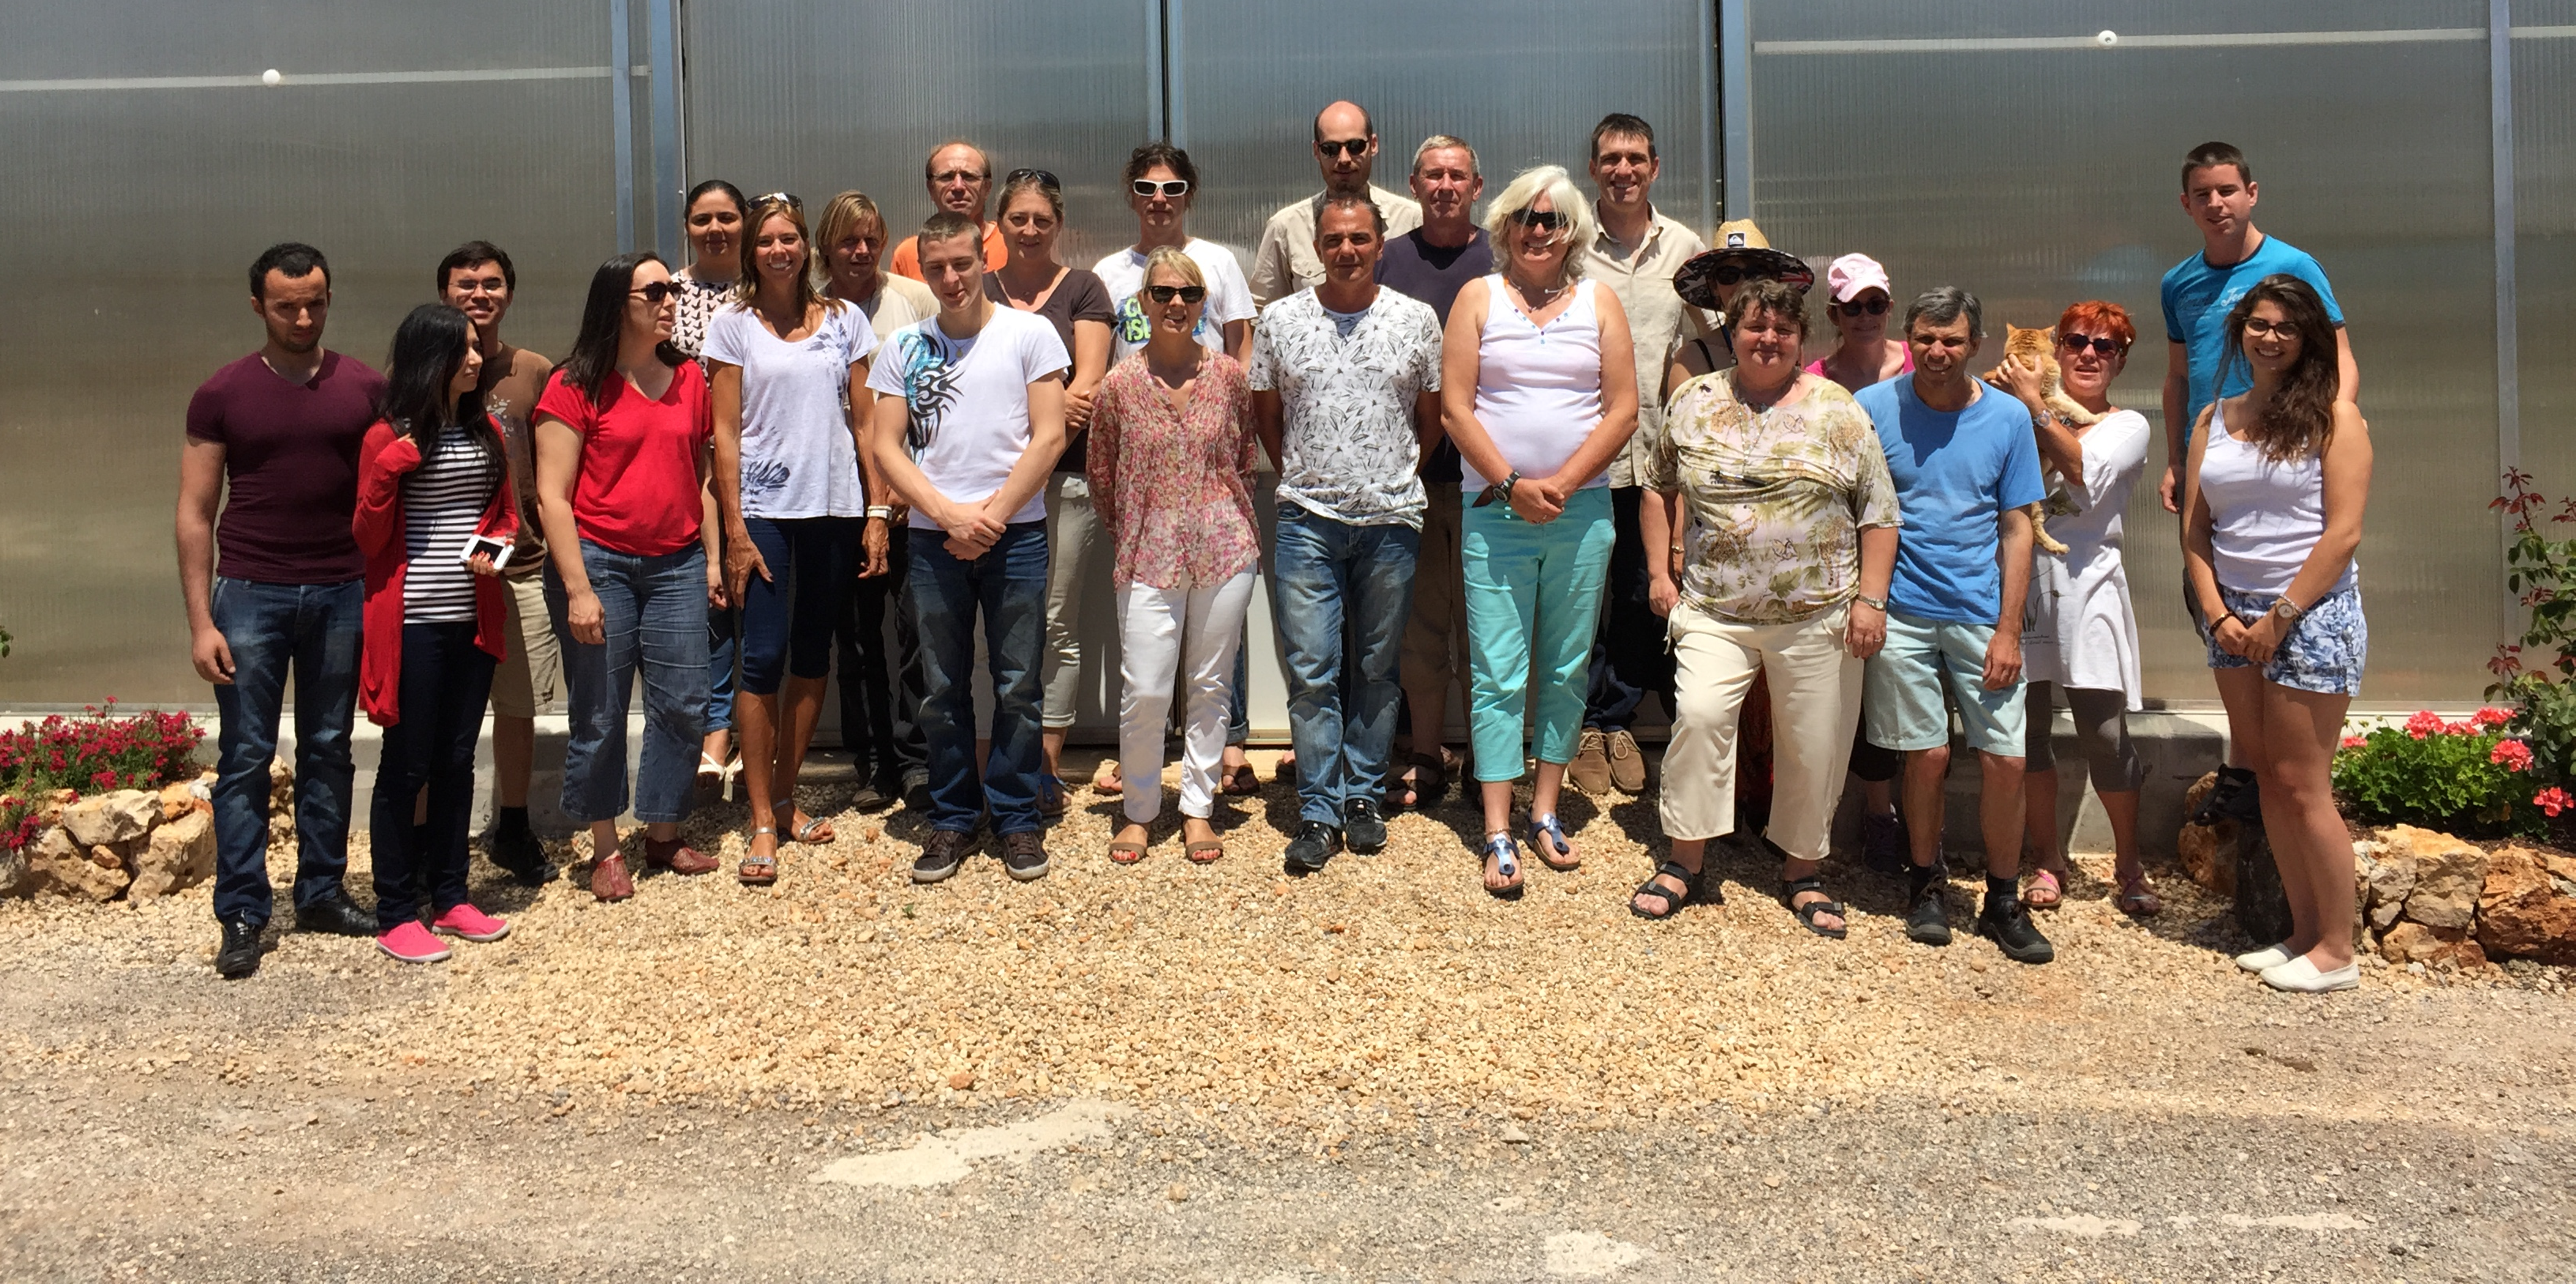
\includegraphics[width =0.8\textwidth]{M2P2} \quad
\centering M2P2
\end{textblock*}




\begin{textblock*}{5cm}(4.15cm,2cm) % {block width} (coords)
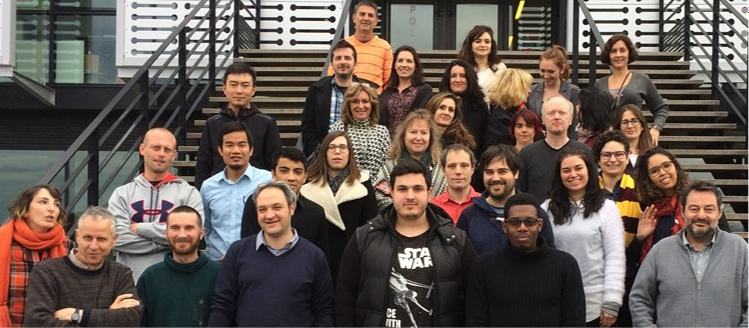
\includegraphics[width =0.9\textwidth]{201707_ipn_samuel.png} \\
\centering IPN
\end{textblock*}


\begin{textblock*}{5cm}(8.2cm,2cm) % {block width} (coords)
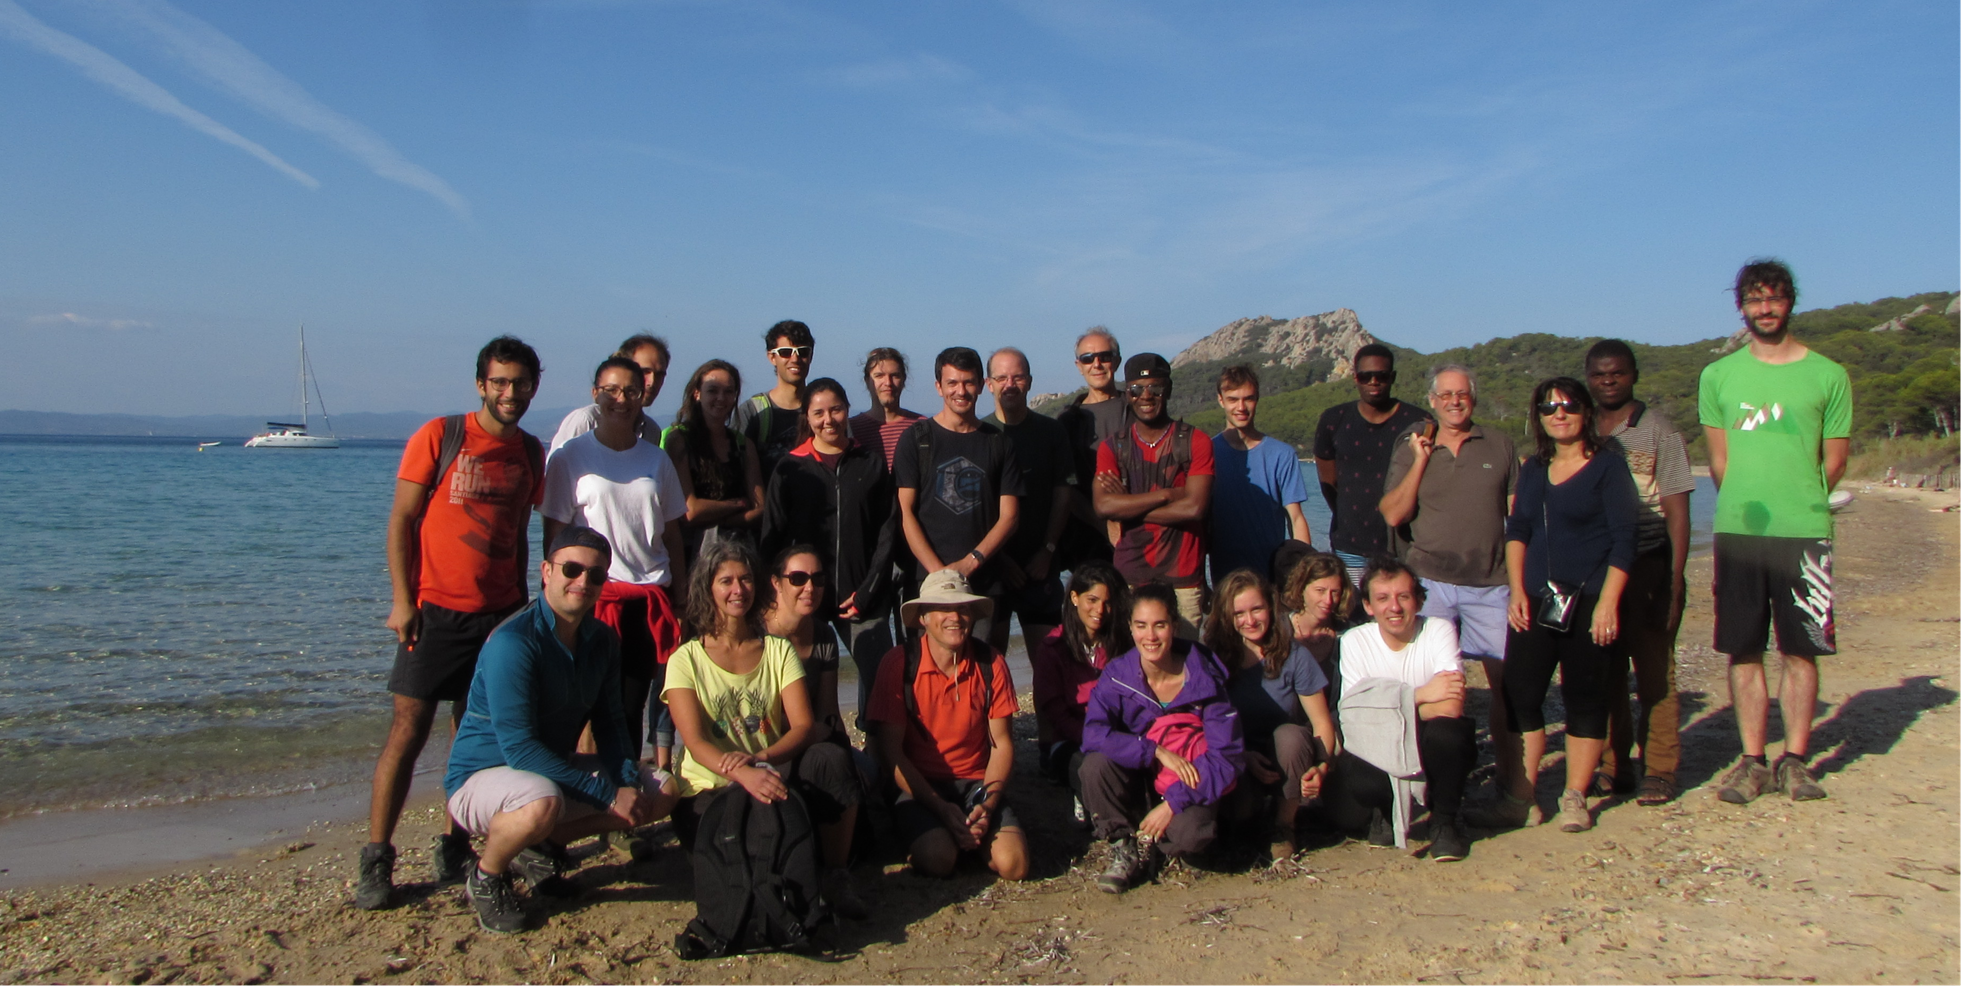
\includegraphics[width =0.8\textwidth]{Seminaire_BIOCORE_2017-10_Porquerolles.png} \quad
\centering BIOCORE
\end{textblock*}

\vspace{40mm}
	\begin{center}
	\textcolor{purple}{\Large\textbf{\textit{Merci de votre attention!}}}\\

	\end{center}
  
\begin{textblock*}{15cm}(2cm,8cm) % {block width} (coords)

\includegraphics[width =0.1\textwidth]{INRAE_logo.png} \quad

\includegraphics[width =0.15\textwidth]{logo-inria.png} \quad

\includegraphics[width =0.05\textwidth]{CNRS_fr_quadri.png} \quad

\includegraphics[width =0.11\textwidth]{paca_logo} \quad

\includegraphics[width =0.1\textwidth]{logo} 
%
\includegraphics[width =.1\textwidth]{logo}
\end{textblock*}

\end{frame}

